\section{KdV equation}
\label{sec:KdV}

\subsection{The model}

\indent The first model of wave propagation studied and implemented in this project is the Korteweg-de Bries (KdV) equation, which takes in account  nonlinear and dispersive effects and is a good approximation for waves with small amplitude and long wavelength.

\indent Different forms of this equation can be found in literature, varying mainly in the scaling factors for each physical process present in the equation (nonlinearity and dispersion). We will consider the formulation derived by \cite{BBM1971}, written in terms of dimensionless but unscaled variables :

\begin{equation}
    u_t + u_x + (u^2)_x + u_{xxx} = 0
\end{equation}

\subsection{Discretization}

\indent The problem to be solved, with a initial condition $\Phi$ and proper boundary conditions, is

\begin{equation}
\begin{cases}
    u_t + u_x + (u^2)_x + u_{xxx} = 0 \ , \ \ x \in [x_{min},x_{max}], \ \ t \in [0, t_{max}] \\
    u(x,0) = \Phi(x) \\
    \text{+ boundary conditions}
\end{cases}
\end{equation}

\indent In a first moment, in order to validate the implementation of the model, without influence of the boundaries, we will consider periodic boundary conditions or, in the nonperiodic case, homogeneous Dirichlet and/or Neumann conditions with the boundaries far enough from the propagating wave.

\indent The numerical resolution will be made with a splitting scheme, separating the advective and the dispersive terms. Therefore, defining the operators


\begin{gather}
	T_a{u} = u_t + u_x + (u^2)_x \\
	T_d{u} = u_t + u_{xxx}
\end{gather}

 
\noindent we will solve, in each time step $[t_n,t_{n+1}]$ :

\begin{equation}
\begin{cases}
   T_a(v) = 0 \ \ ,\ t \in [t_n,t_{n+1}], \  v^n = u^n \\
   T_d(w) = 0 \ \ , \ t \in [t_n,t_{n+1}], \  w^n = v^{n+1} \\
    u^{n+1} = w^{n+1}
\end{cases}
\end{equation}

\indent The numerical schemes used in each of these step is descried below :

\subsubsection{First step}
\label{sec:KdVSplitted1}

\indent The first step of the splitted KdV equation is a hyperbolic conservation law, which can be written in terms of a flux function $f$ :

\begin{equation}
  \label{eq:conservationLaw}
	v_t + f(v)_x = 0, \ \ f(v) = v + v^2
\end{equation}

\indent It will be solved using a Finite Volume method, with the cells $[x_{i-1/2}, x_{i+1/2}]$ centered in the discrete spatial points $x_i$ and with the cell-averaged value of the solution equal to the solution $u_i^n$ in these points. The spatial derivative in \eqref{eq:conservationLaw} will be discretized with a 4th order Runge-Kutta method,

\begin{equation}
\begin{cases}
k_1 = - f(v_i^n)_x \\
k_2 = - f\left(v_i^n + k_1\frac{\Delta t }{2}\right)_x \\
k_3 = - f\left(v_i^n + k_2\frac{\Delta t }{2}\right)_x \\
k_4 = - f(v_i^n + k_3 \Delta t)_x \\
v_i^{n+1} = v_i^n + \frac{\Delta t}{6}(k_1 + 2k_2 + 2k_3 + k_4)
\end{cases}
\end{equation}

\noindent and the spatial derivative will be approximated in terms of the flux on the cells' interfaces : 

\begin{equation}
f(v_i^n)_x = \frac{f\left(v_{i+1/2}^n\right) - f\left(v_{i-1/2}^n\right)}{\Delta x}
\end{equation}

\indent Therefore, we must compute the values of $u$ on each interface. It will be made solving the following Riemann problem :

\begin{equation}
\begin{cases}
v_t + f(v)_x = 0 \\
v(x,0) = v^- \ , \ x < 0 \\
v(x,0) = v^+ \ , \ x > 0
\end{cases}
\end{equation}

\noindent where the boundary is located at $x=0$ and $v^-$ and $v^+$ are the solutions in its two neighbor cells.

\indent The flux function $f$ is uniformly convex, so the Riemann problem has a unique weak, admissible solution \cite{conservationLaws2002} : 

\begin{itemize}
\item  If $v^- > v^+$  (shock) : 
\begin{equation}
v(x,t) = 
\begin{cases}
v^- \ ,\ \   f(v^-) > f(v^+) \\
v^+ \ ,\ \ f(v^-) < f(v^+)
\end{cases}
\end{equation}

\item If $v^+ > v^-$  (rarefaction wave) :
\begin{equation}
v(x,t) = 
\begin{cases}
v^- \ ,\ \ f'(v^-) > 0 \\
\left(f'\right)^{-1}(v) \ ,\ \ f'(v^-) < 0 < f'(v^+) \\
v^+ \ ,\ \ f'(v^+) < 0 
\end{cases}
\end{equation}
\end{itemize}


\subsubsection{Second step}

\indent Two schemes will be proposed for the resolution of the second step of the KdV equation,

\begin{equation}
	\label{eq:dispersion}
	w_t + w_{xxx} = 0
\end{equation}

\noindent depending on the boundary conditions (periodic or not).

\paragraph{Periodic case}

\indent The spatial derivatives and the linearity in the second step \eqref{eq:dispersion} motivates us to implement a Fourier spectral method, which is possible with the periodic boundary conditions. In fact, the method is quite simple :

\indent Let $\hat{w}(k,t_n)$ be the Fourier coefficients of $w(x,t_n)$.  The Fourier transform of the equation \eqref{eq:dispersion} gives

\begin{equation}
	\hat{w}_t(k,t) - ik^3\hat{w}(k,t) = 0
\end{equation}

\indent It is an ODE in $t$,  which solution is

\begin{equation}
\hat{w}(k,t) = e^{ik^3(t-t_n)}\hat{w}(k,t_n)
\end{equation}

\indent Finally, the inverse Fourier transform using the coefficients $\hat{w}(k,t_{n+1})$ gives $w(x,t_{n+1})$

\paragraph{Nonperiodic case}

\indent For this case, the second equation \eqref{eq:dispersion} was solved using an implicit Finite Difference scheme, with fourth order centered discretization of the third spatial derivative, except in the points near the boundaries, for which a simple first order uncentered scheme was used:

\begin{gather}
	\label{eq:IFDSolverKdV}
	\frac{u_i^{n+1} - u_i^n}{\Delta t} + \frac{\frac{1}{8}u_{i-3}^{n+1} - u_{i-2}^{n+1}  + \frac{13}{8}u_{i-1}^{n+1} - \frac{13}{8}u_{i+1}^{n+1} + u_{i+2}^{n+1} - \frac{1}{8}u_{i+3}^{n+1}}{\Delta x^3} = 0, \ \ i = 3,...,N-3 \\
	\frac{u_i^{n+1} - u_i^n}{\Delta t}  + \frac{-u_{i}^{n+1} + 3u_{i+1}^{n+1}  -3 u_{i+2}^{n+1} + u_{i+3}^{n+1} }{\Delta x^3} = 0, \ \ i = 0,1,2 \\
	\frac{u_i^{n+1} - u_i^n}{\Delta t}  + \frac{u_{i}^{n+1} - 3u_{i-1}^{n+1}  + 3 u_{i-2}^{n+1} - u_{i-3}^{n+1} }{\Delta x^3} = 0, \ \ i = N-2,N-1,N \\
\end{gather} 

\noindent which leads to the resolution of a linear system, with the appropriate modifications to take in account the boundary conditions.

\subsubsection{Choice of the time step}

\indent The time step is chosen based on the first step of the splitted equation. In the non-conservative form, the equation \eqref{eq:conservationLaw} is written as

\begin{equation}
v_t +  (1+2v)v_x = 0
\end{equation}

\noindent which configures an advection problem with velocity $1+2v$

\indent The space and time steps must verify the CFL condition : 

\begin{equation}
(1+2v)\frac{\Delta t}{\Delta x} \leq 1
\end{equation}

\noindent in order to avoid non-physical behaviors (e.g. mass increasing). Therefore, for each time step, we will chose, for small $\epsilon$

\begin{equation}
\Delta t = \frac{\Delta x}{1+2\max\limits_{x}|v|} - \epsilon
\end{equation}

\subsection{Scale analysis}

\indent With the objectif of correctly simulating the physical phenomena involved in the KdV equation, the initial solution must satisfy the assumptions made in the derivation of the model. Following this purpose, we perform in the next paragraphs a scale analysis following the arguments presented in \cite{BBM1971}, which at the same time will be linked to the physical case of water surface waves of small amplitude. This analysis will allow us to derive a criteria for selecting the initial conditions of some example simulations. 

\indent We will seek to write the KdV equation in the following dimensionless and scaled form, as described in \cite{BBM1971}

\begin{equation}
\label{eq:scaledKdV}
U_T + U_X + \frac{\epsilon}{2} (U^2)_X + \epsilon\alpha^2U_{XXX} = 0
\end{equation}

\noindent and link it to the parameters involved in the model for surface water waves  in dimensional form \cite{Khorsand2014}

\begin{equation}
    u^*_{t^*} + c_0u^*_{x^*} + \frac{3}{4}\frac{c_0}{h_0}({u^*}^2)_{x^*} + \frac{1}{6}c_0h_0^2u^*_{x^*x^*x^*} = 0 
\end{equation}

\noindent where the $\cdot^*$ denotes the physical variables, $h_0$ the undisturbed water depth for flat bottom and $c_0 = \sqrt{gh_0}$  the long wave speed.

\subsubsection{Characterization of the nonlinearity}

\indent According to \cite{BBM1971}, nonlinearity is characterized by a parameter $\epsilon$ such that if characteristics are written in the form

$$ \frac{1}{c_0} \frac{dx}{dt} = 1+ bu$$

\noindent then one can choose an $\epsilon \ll 1$ such that $bu=\epsilon U$, with $U$ of order one. For the particular case of water waves this can be represented as

$$ \frac{1}{c_0} \frac{dx}{dt} = 1 + \frac{3}{2h_0}u$$

\noindent and thus $b = \frac{3}{2h_0}$. This parameter will be used in the next arguments.

\subsubsection{Characterization of the dispersion}

\noindent The characterization of the dispersion comes from the derivation of the KdV equation. According to \cite{BBM1971} if the propagation of the wave follows a law of the form

$$ u^*_{t^*} + uu_x+(\mathcal{L} u^*)_{x^*} = 0$$

\noindent with $\mathcal{L}$ such that $$ \widehat{\mathcal{L}u^*} = \frac{c(k)}{c_0} \widehat{u^*}(k,t)$$ with $\hat \cdot$ the Fourier transform and $c(k)$ the phase celerity, which is equivalent to 

$$ \mathcal{L} u = \mathcal{F}^{-1}\left(\frac{c(k)}{c_0}\right) * u$$ 

\noindent where $\mathcal{F}^{-1}$ is the inverse Fourier transform operator, then new scaling based on the fact that for $\kappa$ sufficiently small, the wave speed $c(\kappa) = c_0 + c_0 \sum_{n=1}^{\infty}A_n\epsilon^n\kappa^{2n}$ can be approximated by $c(\kappa) = c_0(1-\kappa^2)$, which motivates replacing $x=\sqrt{\epsilon} X$, $t =c_0 \sqrt{\epsilon} T$, and $u = \frac{\epsilon}{ b} U$ to obtain the equivalent equation 

$$ U_T + \epsilon U U_x+(\mathcal{L}_{\epsilon} U)_{X} = 0$$

\noindent with $\mathcal{L}_\epsilon$ such that 

$$ \widehat{\mathcal{L}_\epsilon U} = \frac{c(\epsilon^{1/2} K)}{c_0} \hat{U}(K,T)$$ 

\noindent with $K=\sqrt{\epsilon} k$, which after replacing the full series expansion of $c(k)$ leads to

\begin{align}
  \label{eq:expansionLe}
    \mathcal{L}_\epsilon U &=U +\sum_{n=1}^\infty (-1)^n A_n \epsilon^n \partial_X^{2n} U    
\end{align}

\noindent and if terms for $n\geq2$ are neglectable, which is the case for $\epsilon \ll 1 $ and if one supposes that all derivatives of $U$ are of the same order of magnitude, then one obtains that

\begin{align*}
    \mathcal{L}_\epsilon U &= U + A_n \epsilon \frac{\partial^2 U}{\partial x^2} \\
    &= U - \alpha^2 \epsilon \frac{\partial^2 U}{\partial x^2} \\
\end{align*}

\noindent with $\alpha^2 = - A_n$. Replacing in the scaled equation results in

$$U_T + U_X + \frac{\epsilon}{2} (U^2)_X + \epsilon\alpha^2U_{XXX} = 0$$

\indent Applying the same scaling $x=\sqrt{\epsilon} X$, $t =c_0 \sqrt{\epsilon} T$, and $u = \frac{\epsilon}{ b} U$ to the physical equation leads to $$U_T + U_X + \frac{3\epsilon}{4b} (U^2)_X + \frac{h_0^2\epsilon}{6}U_{XXX} = 0$$
from where, comparing to \eqref{eq:scaledKdV}, one concludes that $ \alpha^2 = \frac{h_0^2}{6} $

\subsection{The criteria}

\subsubsection{Choice of the wavelength}

\indent A sufficient condition for the terms of order greater than 1 in the power series expansion of $\mathcal{L}_\epsilon$  (equation \eqref{eq:expansionLe}) to be neglectable is that those terms are also neglectable for $c(k)$, given that that all the derivatives of $U$ have an order of magnitude 1.

\indent A key point in the derivation of the KdV equation is to assure that the terms for the higher derivatives (for $n > 1$) are small enough to be neglected. Firstly, \cite{BBM1971} assumes that all this derivatives have have an order of magnitude 1. Secondly, a sufficient condition for this is that those terms are also neglectable in the series expansion of $c(k)$. Thirdly, also accordingly to \cite{BBM1971}, the following form is applicable to surface waves : 

$$c(\kappa) = c_0 \left(\frac{tanh(\kappa h_0)}{\kappa h_0}\right) = c_0 \left(1 - \frac{1}{6}(\kappa h_0)^2 + \frac{19}{360}(\kappa h_0)^2 + ... \right) $$

\noindent from where we can see that we must choose $\kappa h_0 \ll 1$

\indent Denoting $\lambda$ as the wavelength, and choosing a constant $B$ such that $\kappa h_0  =  B \ll 1$, it follows that $h_0 = \frac{B\lambda}{2\pi}$, and, from the relation $\alpha^2 = \frac{h_0^2}{6}$, we get $\alpha^2 = \frac{B^2\lambda^2}{6(2\pi)^2}$.

\subsubsection{Choice of the wave amplitude}

\indent From $bu^* = \epsilon U$, with $U$ of unit order magnitude, and since $b = \frac{3}{2h_0}$, the physical variable is written as $u^* = \frac{2}{3}h_0\epsilon U, \ (\epsilon > 0)$, thus if $\epsilon$ represents the amplitud of the wave, $\frac{2}{3}\epsilon h_0$ is the wave amplitude (as done in the scale study). Accordingly to \cite{BBM1971}, the nonlinearity in the KdV equation is valid for $\epsilon \ll 1$. Therefore, $\epsilon$ will be chosen taking in account this condition.

\subsubsection{Resume}

\indent In resume, the proposed criteria to construct the initial data is : 

\begin{enumerate}
\item Adopt a water depth $h_0$ (e.g. from the data)
\item Choose a wave amplitude  $A = \frac{2}{3}h_0\epsilon$, then the restriction $\epsilon \ll 1$ translates to $\frac{A}{h_0} = \frac{2}{3}\epsilon \ll 1$.
\item Choose a wavelength $\lambda$ such that $\kappa h_0 = \frac{2\pi}{\lambda}h_0 = B \ll 1$, which translates to $\frac{h_0}{\lambda} = \frac{B}{2\pi} \ll 1$
\item The effect of dispersion over non linearity can be measured by taking the quotient of their coefficients $\frac{\epsilon \alpha^2}{\epsilon} = \alpha^2$.
\end{enumerate}

\indent From another point of view, one can define a wave of amplitude $A$ and wavelength $\lambda$ and compute the range of depths in which this initial condition is valid, for a given precision : 

\begin{equation} 
\label{eq:hvalid}
h_0^{valid} = \left[ \frac{3A}{2\epsilon}, \frac{B\lambda}{2\pi}\right]
\end{equation}

\indent This is consistent with the fact that the KdV model is valid for waves with small amplitude and large wavelenght \cite{BBM1971}.

\subsubsection{Examples}

\indent We present here twwo examples to test the proposed numerical solution for the KdV equation. These examples are inspired in those showed in \cite{conservationLaws2002}: the initial solutions are gaussian waves (far enough from the boundaries in order to avoid its influence) with different amplitude and wavelength (the wavelength is adopted as the standard deviation). The idea is to verify the influence of these characteristics on the nonlinear and dispersive effects, and also to check the water depth range in which the propagation of this solution can be modeled by the KdV equation.  Both tests were made with $B = 0.1$ and $\epsilon = 0.001$.

\indent The initial solutions used are

\begin{enumerate}
	\item \textbf{Short wave (figure \ref{fig:KdVcriteriaShort})} % Criteria 6
		\begin{itemize}
			\item $\lambda = 1$
			\item $ A = 10^{-5}$
			\item $ h_0^{valid} = [0.15, 0.16] $
		\end{itemize}
	\item \textbf{Long wave (figure \ref{fig:KdVcriteriaLong})} % Criteria 5
		\begin{itemize}
			\item $\lambda = 250000$
			\item $ A = 0.1$
			\item $ h_0^{valid} = [150, 3979] $
		\end{itemize}
\end{enumerate}

\begin{figure}[h]
	\begin{subfigure}{.5\linewidth}
		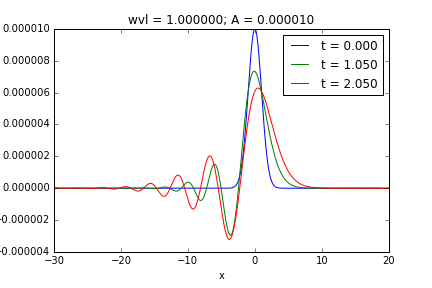
\includegraphics[scale=.45]{figures/criteria6.png}
		\caption{Short gaussian wave 		\label{fig:KdVcriteriaShort}}
	\end{subfigure}
	\begin{subfigure}{.5\linewidth}
		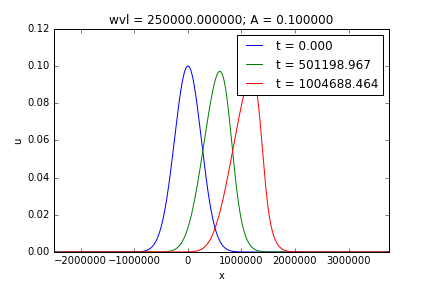
\includegraphics[scale=.45]{figures/criteria5.png}
		\caption{Long gaussian wave		\label{fig:KdVcriteriaLong}}
	\end{subfigure}
	\caption{Simulations with the KdV equation 	\label{fig:KdVcriteria}}
\end{figure}

\paragraph{Conclusions :}

\begin{itemize}
 \item These results are compatible with the observations and examples made by \cite{conservationLaws2002}, which states that dispersive effects are stronger in shorter waves; in the long wave, the nonlinear effect is more evident.
 \item The range of validity of the KdV equation is very small in the case of the short wave, and much larger for the long wave. This is coherent with the fact that this model is a good approximation for the propagation of long waves with small finite amplitude, which can be seen in the definition of $h_0^{valid}$ (equation \eqref{eq:hvalid}) : reducing $A$ and increasing $\lambda$ increases the length of the interval of validity.
 \item One of our conclusions in the derivation of the proposed criteria should be revised : the one which says that the importance of the dispersive over the nonlinear effects can be measured by $\alpha^2 = \frac{h_0^2}{6}$ : in fact, in the given examples, if we adopt $h_0$ as the median of $ h_0^{valid} $, the highly-dispersive short wave has a smaller $\alpha^2$ than the long wave.
\end{itemize} 